%% 
%% Latex Practice
%% Use https://tikzcd.yichuanshen.de/ for diagrams
%leqno,fleqn,
\documentclass[10pt,letterpaper]{article}


\usepackage[comma,authoryear]{natbib}
\usepackage{float}
\usepackage{graphicx}
\usepackage{setspace}
% \usepackage{kpfonts}
\usepackage{textcomp}
% \usepackage{fullpage}
\usepackage{url}
\usepackage[usenames,dvipsnames,svgnames,table]{xcolor}
%\usepackage{mdframed}  % not availble on ubuntu

% -- font styles
\usepackage{tgtermes}
% \usepackage[lf]{venturis}
% \usepackage{times}
% \usepackage[sc]{mathpazo} % Palatino (very readable)
% \usepackage[adobe-utopia]{mathdesign}
% \usepackage{gfsdidot}
% \usepackage[scaled]{beraserif}
% \usepackage[bitstream-charter]{mathdesign}
% \usepackage{mathptmx}
\usepackage{enumitem}
% some more math stuff/ diagrams
\usepackage{amssymb}
\usepackage{tikz-cd}
% special math formatting
\usepackage{amsmath}

\floatstyle{ruled}

% -- structural elements
\newfloat{program}{thp}{lop}
\floatname{program}{Program}

%\newfloat{figure}{thp}{lop}
%\floatname{figure}{Figure}

% -- syntax highlighting
\usepackage{listings}
  \usepackage[scaled]{beramono}
  \usepackage[T1]{fontenc}
\usepackage{color}

\usepackage{caption}
% -- configure captions for figures
\DeclareCaptionFormat{listing}{\par\hrule #1#2#3}
\captionsetup[figure]{%
  format=listing, 
  singlelinecheck=false, 
  margin=00pt, 
  font={it,footnotesize,centering}
}

\parskip 12pt

% page margins
\setlength{\textheight}{22cm}
\setlength{\oddsidemargin}{0.25in}
\setlength{\textwidth}{6in}

% I don't know what this does
\def\printcitestart{\unskip $^\bgroup}
\def\printbetweencitations{,}
\def\printcitefinish{\egroup$}
\def\printcitenote#1{\hbox{\sevenrm\space (#1)}}


% TODO: mdframed doesn't work well with ubuntu
% \newenvironment{aside}
%   {\begin{mdframed}[style=0,%
%       leftline=false,rightline=false,leftmargin=2em,rightmargin=2em,%
%           innerleftmargin=0pt,innerrightmargin=0pt,linewidth=0.75pt,%
%       skipabove=25pt,skipbelow=25pt]\small}
%   {\end{mdframed}}


%% Bibliography configuration
%% ------------------------------
\bibliographystyle{apalike}
% don't show reference label in the bibliography (APA specific)
\makeatletter
\def\@biblabel#1{}
\makeatother


\lstset{
  %framesep=5pt,
  upquote=true,
  breaklines=false,
  %postbreak=\raisebox{0ex}[0ex][0ex]{\ensuremath{\hookrightarrow}},
  breakatwhitespace=true,
  %numbers=left,
  language=Java,
  basicstyle=\footnotesize\ttfamily,
  numberstyle=\footnotesize\ttfamily,
  %numbersep=10pt,
  tabsize=2,
  extendedchars=true,
  showtabs=false,
  showspaces=false,
  showstringspaces=false,
  xleftmargin=20pt,
  aboveskip=10pt,
  % colors
  stringstyle=\color{Maroon},
  commentstyle=\color{Gray},
  rulecolor=\color{Gray},
  keywordstyle=\color{Blue},
  %backgroundcolor=\color{LightGray!.50}
}
\lstloadlanguages{
  Java
}


% Hyphenation rules ------------
%% \hyphenation{Fire-Detection-System}
%% \hyphenation{Emergency-Communication-System}


\title{Algorithm Design Manual Notes}
\author{Zachary William Grimm\\
  \small{Notes  for ADM by Skiena}\\
  \small{zwgrimm@gmail.com}
}
\date{\today{}}

\begin{document}

\setstretch{1.00}
\maketitle

% -- Table of Contents --
\tableofcontents{}

\newpage{}

% -- set document spacing --
% \setstretch{1.09}  % single line
% \setstretch{1.30}  % single wide-spaced\subsubsection*{\textbf{1-12.} \emph{Prove that $\sum_{i=1}^{n}i^{3}=\frac{n^{2}(n+1)^{2}}{4} \;for\; n \geq 0$, by induction}}
% \setstretch{1.50}  % one and a half spacing

% -- Import content here
\section{Introduction To Algorithm Design}
the algorithmic \emph{problem} known as \emph{sorting} is defined as follows: \\
\emph{Problem:} Sorting \\
\emph{Input:} A sequence of n keys $a_{1},...,a_{n}$. \\
\emph{Output:} The permutation (reordering) of the input sequence such that $a_{1}^{'} \leq a_{2}^{'} \leq ... \leq a_{n-1}^{'} \leq a_{n}^{'}$\\


\noindent\rule{\textwidth}{0.4pt}

\begin{figure}[H]
  \centering
     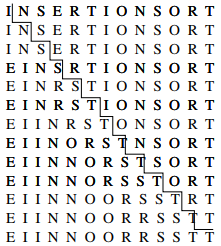
\includegraphics[scale=0.6]{./insertion_sort.png}
  \label{fig:demo-diagram}
  \caption{Animation of insertion sort in action (time flows down)}
\end{figure}


\begin{verbatim}
insertion_sort(item s[], int n)
{
    int i,j; /* counters */

    for (i=1; i<n; i++) {
        j=i;
        while ((j>0) && (s[j] < s[j-1])) {
            swap(&s[j], &s[j-1]);
            j = j-1;
        }
    }
}
\end{verbatim}

\noindent\rule{\textwidth}{0.4pt}


\begin{figure}[H]
  \centering
     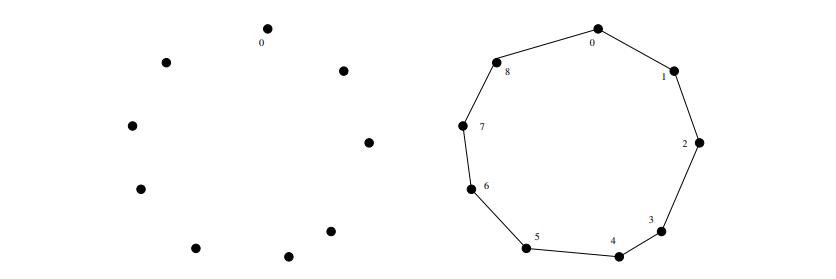
\includegraphics[scale=0.6]{./nearest_neighbor.png}
  \label{fig:demo-diagram2}
  \caption{A good instance for the nearest neighbor heuristic}
\end{figure}




\subsection{Robot Tour Optimization}
aaa
\subsection{Selecting the Right Jobs}
bbb

\subsubsection{test, delete this}
\subsection{Reasoning about Correctness}

\subsubsection{Expressing Algorithms}









% -- Bibliography (APA)
% \bibliography{references}

\end{document}